\documentclass[12pt,a4paper]{article}

\usepackage[utf8]{inputenc}
\usepackage[french]{babel}
\usepackage[T1]{fontenc}

\usepackage{amsmath}
\usepackage{amsfonts}
\usepackage{amssymb}

% Preparation des infos generales
\newcommand{\TitreMatiere}{Rattrapages Python}
\newcommand{\DateExo}{27 juin 2022}
\newcommand{\TypeExo}{Rattrapage}
\newcommand{\TitreExercice}{Code Python}
\newcommand{\NomAuteurA}{Mark ANGOUSTURES}
\newcommand{\MailAuteurA}{mark.angoustures@epita.fr}
%\newcommand{\NomAuteurB}{ }
%\newcommand{\MailAuteurB}{ }
\newcommand{\VersionExo}{Version 1}
\newcommand{\LoginEtudiant}{2021-2022} % Watermark de protection

%\newcommand{\RenduTarball}{nom1-nom2-TP1.tar.bz2}
%\newcommand{\RenduDir}{nom1-nom2-TP1}
\newcommand{\RenduTarball}{login-RATT-Python.tar.bz2}
\newcommand{\RenduDir}{login-RATT-Python}


% Ajout de mes classes & definitions
\usepackage{MetalExo} % Appelle un .sty


% Redefinition headers
\lhead{\TitreExercice}		%Gauche Haut
\chead{\TypeExo}			%Centre Haut
\rhead{\thepage}			%Droite Haut
\lfoot{}					%Gauche Bas
\cfoot{\TitreMatiere}		%Centre Bas
\rfoot{}					%Droite Bas


\definecolor{mygreen}{rgb}{0,0.6,0}		% RGB model
\definecolor{mygray}{rgb}{0.5,0.5,0.5}
\definecolor{mymauve}{rgb}{0.58,0,0.82}


\usepackage{array}
\newcolumntype{P}[1]{>{\raggedright\arraybackslash }m{#1}}

\newcolumntype{R}[1]{>{\raggedleft\arraybackslash }b{#1}}
\newcolumntype{L}[1]{>{\raggedright\arraybackslash }b{#1}}
\newcolumntype{C}[1]{>{\centering\arraybackslash }b{#1}}

\newcolumntype{M}[1]{>{\raggedright\let\newline\\\arraybackslash\hspace{0pt}}m{#1}} % another L
\newcolumntype{D}[1]{>{\centering\let\newline\\\arraybackslash\hspace{0pt}}m{#1}}   % another C
\newcolumntype{S}[1]{>{\raggedleft\let\newline\\\arraybackslash\hspace{0pt}}m{#1}}  % another R

\begin{document}

%% Titre
\maketitle

%\newpage

%% Copyright
\pagenumbering{Roman}

%% Copyright

{\Large \textbf{Copyright}}

\vspace{30px}

Ce document est destiné à l'usage interne de Paris 1 - Panthéon Sorbonne.\\

Copyright \space \copyright \space Fabrice BOISSIER - 2019\\

\bigskip

\begin{center}
	\fcolorbox{black}{white}{\makebox[14cm]{
	\begin{minipage}[l]{12cm}
		\vspace*{10px}
		\textbf{Ce document est soumis à conditions :}
		\medskip

		Il est interdit de partager ce document avec d'autres personnes.
		\smallskip

		Vérifiez que vous disposez de la dernière révision de ce document.
	\vspace*{10px}
	\end{minipage}
	}}
\end{center}


\newpage

%% Table des matieres
\tableofcontents

\newpage

%% Consignes generales
\section{Consignes Générales}

\bigskip

%% Consignes generales
\noindent \textit{Les informations suivantes sont très importantes :}

\bigskip

\noindent \textit{Le non-respect d'une des consignes suivantes entraînera des sanctions pouvant aller jusqu'à la multiplication de la note finale par 0.}

\bigskip

\noindent \textit{Ces consignes sont claires, non-ambiguës, et ont un objectif précis. En outre, elles ne sont pas négociables.}

\bigskip

\noindent N'hésitez pas à demander si vous ne comprenez pas une des règles.

\bigskip

\newcounter{My_Counter}

\ConsigneGenerale{My_Counter}{Vous devez lire le sujet.}
\ConsigneGenerale{My_Counter}{Vous devez respecter les consignes.}
\ConsigneGenerale{My_Counter}{Vous devez rendre le travail dans les délais prévus.}

\medskip

\ConsigneGenerale{My_Counter}{Le travail doit être rendu dans le format décrit à la section \hyperref[sec:FormatDeRendu]{Format de Rendu}.}

\ConsigneGenerale{My_Counter}{Le travail rendu ne doit pas contenir de fichiers binaires, temporaires, ou d'erreurs (\texttt{\textbf{*\textasciitilde}}, \texttt{\textbf{*.o}}, \texttt{\textbf{*.a}}, \texttt{\textbf{*.so}}, \texttt{\textbf{*\#*}}, \texttt{\textbf{*core}}, \texttt{\textbf{*.log}}, \texttt{\textbf{*.exe}}, binaires, ...).}

\ConsigneGenerale{My_Counter}{Dans l'ensemble de ce document, la casse (caractères majuscules et minuscules) est très importante. Vous devez strictement respecter les majuscules et minuscules imposées dans les messages et noms de fichiers du sujet.}

%\ConsigneGenerale{My_Counter}{Dans l'ensemble de ce document, \LoginX \space correspond à votre login.}
\ConsigneGenerale{My_Counter}{Dans l'ensemble de ce document, \TTBF{nom1-nom2} \space correspond à la combinaison des deux noms de votre binôme (par exemple pour Fabrice BOISSIER et Mark ANGOUSTURES, cela donnera \TTBF{boissier-angoustures}).}

\ConsigneGenerale{My_Counter}{Dans l'ensemble de ce document, le caractère \TTBF{\textvisiblespace } correspond à une espace (s'il vous est demandé d'afficher \TTBF{\textvisiblespace \textvisiblespace \textvisiblespace }, vous devez afficher trois espaces consécutives).}

\ConsigneGenerale{My_Counter}{Tout retard, même d'une seconde, entraîne la note non négociable de 0.}

\ConsigneGenerale{My_Counter}{La triche (échange de code, copie de code ou de texte, ...) entraîne \textbf{au mieux} la note non négociable de 0.}

\ConsigneGenerale{My_Counter}{En cas de problème avec le projet, vous devez contacter le plus tôt possible les responsables du sujet aux adresses mail indiquées.}

\bigskip

\noindent \textbf{Conseil :} N'attendez pas la dernière minute pour commencer à travailler sur le sujet.


\newpage

%% Format de Rendu
\section{Format de Rendu}
\label{sec:FormatDeRendu}

\vspace*{1cm}

%% Format de Rendu

%\ResponsablesProjet{Metal Man/metalman@example.org, Damdoshi/damdoshi@example.org, Tayst/tayst@tayst.org}
%\begin{tabular}{p{7cm} p{10cm}}
\begin{tabular}{p{7cm} p{8.5cm}}
	%\ResponsablesProjetRow{Fabrice BOISSIER/fabrice.boissier@univ-paris1.fr, Ali JAFFAL/ali.jaffal@univ-paris1.fr}
	\ResponsablesProjetRow{Fabrice BOISSIER/fabrice.boissier@epita.fr}
	& \\
%	\RenduSpecsGenerales{[PHP][DM]}{2}{Envoi par mail}{\RenduDir}{\RenduTarball}{10/02/2020 23h42}{2 semaines}
%	\RenduSpecsGenerales{[CAV][TP1]}{1}{Pas de rendu}{\RenduDir}{\RenduTarball}{Pas de rendu}{Pas de rendu}
	\RenduSpecsGenerales{[C][STR]}{1}{Devoir/Assignment sur Teams}{\RenduDir}{\RenduTarball}{18/12/2022 23h42}{2 semaines}
	& \\
%	\RenduSpecsTechniques{WAMP ou MAMP}{PHP}{Apache/PHP}{ }
%	\RenduSpecsTechniques{Linux - Ubuntu (x86\_64)}{C}{/usr/bin/gcc}{-W -Wall -Werror -std=c99 -pedantic}
	\RenduSpecsTechniques{Linux}{C}{gcc}{-W -Wall -Werror -std=c99 -pedantic}
%	& \\
%	Fonctions autorisées : & malloc(3), free(3), printf(3)
\end{tabular}


\vspace*{1cm}


\noindent Les fichiers suivants sont requis :

\medskip

\begin{tabular}{l p{12cm}}
\texttt{AUTHORS} & contient le(s) nom(s) et prénom(s) de(s) auteur(s).\\
%\texttt{Makefile} & le Makefile principal.\\
\texttt{README} & contient la description du projet et des exercices, ainsi que la fa\c con d'utiliser le projet.\\
%\texttt{configure} & le script shell de configuration pour l'environnement de compilation.\\
\end{tabular}


\vspace*{1cm}


%\noindent Un fichier \TTBF{Makefile} doit être présent à la racine du dossier, et doit obligatoirement proposer ces règles :

\medskip

%\begin{tabular}{l p{13cm}}
%\texttt{all} & \textit{[Première règle]} lance la règle \texttt{libmyqueue}.\\
%\texttt{clean} & supprime tous les fichiers temporaires et ceux créés par le compilateur.\\
%\texttt{dist} & crée une archive propre, valide, et répondant aux exigences de rendu.\\
%\texttt{distclean} & lance la règle \texttt{clean}, puis supprime les binaires et bibliothèques.\\
%\texttt{check} & lance le(s) script(s) de test.\\
%\texttt{libmyqueue} & lance les règles \texttt{shared} et \texttt{static} \\
%\texttt{shared} & compile l'ensemble du projet avec les options de compilations exigées et génère une bibliothèque dynamique.\\
%\texttt{static} & compile l'ensemble du projet avec les options de compilations exigées et génère une bibliothèque statique.\\
%\end{tabular}


%\vspace*{1cm}
%\newpage

\noindent Votre code sera testé automatiquement, vous devez donc scrupuleusement respecter les spécifications pour pouvoir obtenir des points en validant les exercices.
%
Votre code sera testé en l'intégrant à une série de tests automatisés qui seront fournis un peu plus tard.
N'attendez SURTOUT PAS que ces tests soient envoyés pour commencer à produire vos fonctions et vos propres tests.
%
%Votre code sera testé en générant un exécutable ou des bibliothèques avec les commandes suivantes :

%\medskip
%
%\begin{tabular}{l}
%\texttt{./configure}\\
%\texttt{make}\\
%\end{tabular}
%
%\bigskip
%
%\noindent Suite à cette étape de génération, les exécutables ou bibliothèques doivent être placés à ces endroits :
%
%\medskip
%
%\begin{tabular}{l}
%\TTBF{\RenduDir/libmyqueue.a}\\
%\TTBF{\RenduDir/libmyqueue.so}\\
%\end{tabular}

\bigskip

\noindent L'arborescence attendue pour le projet est la suivante :

\medskip

\begin{tabular}{l}
\TTBF{\RenduDir/}\\
\TTBF{\RenduDir/AUTHORS}\\
\TTBF{\RenduDir/README}\\
%\TTBF{\RenduDir/Makefile}\\
%\TTBF{\RenduDir/configure}\\
%\TTBF{\RenduDir/check/}\\
%\TTBF{\RenduDir/check/check.sh}\\
\TTBF{\RenduDir/src/}\\
\TTBF{\RenduDir/src/StrBasics.c}\\
\TTBF{\RenduDir/src/StrBasics.h}\\
\TTBF{\RenduDir/src/StrPart1.c}\\
\TTBF{\RenduDir/src/StrPart1.h}\\
\TTBF{\RenduDir/src/StrPart2.c}\\
\TTBF{\RenduDir/src/StrPart2.h}\\
%\TTBF{\RenduDir/src/StrBonus.c}\\
%\TTBF{\RenduDir/src/StrBonus.h}\\
\end{tabular}


\vspace*{1cm}


%\noindent \textit{Vous ne serez jamais pénalisés pour la présence de makefiles ou de fichiers sources (code et/ou headers) dans les différents dossiers du projet tant que leur existence peut être justifiée (des makefiles vides ou jamais utilisés sont pénalisés).}

%\noindent \textit{Vous ne serez jamais pénalisés pour la présence de fichiers de différentes natures dans le dossier \texttt{check} tant que leur existence peut être justifiée (des fichiers de test jamais utilisés sont pénalisés).}


%%%%%%%%%%%%%%%%%%%%%%%%%%%%
%% AIDE MEMOIRE AU CAS OU %%
%%%%%%%%%%%%%%%%%%%%%%%%%%%%
\newpage

\section{Aide Mémoire}
\label{sec:AideMemoire}

\vspace*{1cm}

%%%%%%%%%%%%%%%%%%%%%%%%%%%%
%% AIDE MEMOIRE AU CAS OU %%
%%%%%%%%%%%%%%%%%%%%%%%%%%%%
%\newpage

%{\Large \textbf{Aide Mémoire}}

%\vspace{30px}

%\noindent Le travail doit être rendu au format \textbf{\textit{.zip}}, c'est-à-dire une archive \textbf{zip} compressée avec un outil adapté (les logiciels \textit{7zip} ou \textit{Keka} sont gratuits et adaptés).
\noindent Le travail doit être rendu au format \textbf{\textit{.tar.bz2}}, c'est-à-dire une archive \textbf{bz2} compressée avec un outil adapté (voir \TTBF{man 1 tar} et \TTBF{man 1 bz2}).

%\noindent Tout autre format d'archive (rar, 7zip, gz, gzip, bzip, ...) ne sera pas pris en compte, et votre travail ne sera pas corrigé (entraînant la note de 0).
\noindent Tout autre format d'archive (zip, rar, 7zip, gz, gzip, ...) ne sera pas pris en compte, et votre travail ne sera pas corrigé (entraînant la note de 0).

\bigskip

\noindent Pour générer une archive \textit{tar} en y mettant les dossiers \textit{folder1} et \textit{folder2}, vous devez taper :

\TTBF{tar cvf MyTarball.tar folder1 folder2}


\bigskip


\noindent Pour générer une archive \textit{tar} et la compresser avec GZip, vous devez taper :

\TTBF{tar cvzf MyTarball.tar.gz folder1 folder2}


\bigskip


\noindent Pour générer une archive \textit{tar} et la compresser avec BZip2, vous devez taper :

\TTBF{tar cvjf MyTarball.tar.bz2 folder1 folder2}


\bigskip


\noindent Pour lister le contenu d'une archive \textit{tar}, vous devez taper :

\TTBF{tar tf MyTarball.tar.bz2}


\bigskip


\noindent Pour extraire le contenu d'une archive \textit{tar}, vous devez taper :

\TTBF{tar xvf MyTarball.tar.bz2}


\vspace*{1cm}

%\noindent Dans ce sujet précis, vous ferez du code en C et des appels à des scripts shell qui afficheront les résultats dans le terminal (donc des flux de sortie qui pourront être redirigés vers un fichier texte).

%\noindent Dans ce sujet précis, vous ferez du code en script shell, qui affichera les résultats dans le terminal (donc des flux de sortie qui pourront être redirigés vers un fichier texte).

%\noindent Dans ce sujet précis, vous ferez du code en PHP, qui affichera les résultats dans une page HTML. Les valeurs seront affichées dans une \textit{textarea} dont le texte est généré par des outils multiplateformes supportant les retours à la ligne UNIX (\textbf{\textbackslash n}). Il ne faut donc pas inclure de balise \TTBF{"<br />"} pour retourner à la ligne, mais un \TTBF{"\textbackslash n"}.

\noindent Dans ce sujet précis, vous ferez du code en Python, qui affichera les résultats dans le terminal (donc des flux de sortie qui pourront être redirigés vers un fichier texte).

%\vspace*{1cm}

%\noindent Pour réaliser le travail demandé, nous vous fournirons pour chaque exercice au moins 2 fichiers : \TTBF{exoN\_res.php} (le fichier qui sera appelé pour voir le résultat de votre travail), et \TTBF{exoN\_fun.php} (le fichier contenant la fonction que vous devez coder dans chaque exercice).
%Optionnellement, un fichier \TTBF{exoN\_data.php} peut être fourni pour indiquer le format de données en entrée.
%Le \TTBF{N} correspond au numéro de l'exercice.

%\medskip

%\noindent Dans tous les cas, vous ne devez rendre que le fichier \TTBF{exoN\_fun.php} avec au moins la fonction demandée remplie (qui peut faire appel à d'autres fonctions que vous définirez dans le \textbf{même} fichier). Les autres fichiers seront générés par nos soins pour tester vos fonctions.

%\vspace*{1cm}

%\noindent Vous ne devez \textbf{PAS} utiliser la fonction \TTBF{echo} pour écrire !
%Il faut retourner une chaîne de caractères correctement formattée.


\newpage

\pagenumbering{arabic}

%%%%%%%%%%%%%%%
%%   COURS   %%
%%%%%%%%%%%%%%%
%\section{Cours}
%
%\vspace*{0.7cm}
%
%\newcommand{\defaultparindent}{\parindent}
\setlength{\parindent}{0pt}				% \noindent partout
% \parindent in one-column documents is :
% 15pt when the default text size is 10pt,
% 17pt for 11pt,
% and 1.5em for 12pt.
% In two-column documents it is 1em

%\begin{center}
%\begin{tabular}{p{5cm} p{11cm}}
%\textbf{Commandes étudiées :} & \texttt{sh}, \texttt{bash}, \texttt{man}, \texttt{ls}, \texttt{mkdir}, \texttt{touch}, \texttt{chmod}, \texttt{mv}, \texttt{rm}, \texttt{rmdir}, \texttt{cat}, \texttt{file}, \texttt{whereis}, \texttt{which}\\

%\textbf{Builtins étudiées :} & \texttt{pwd}, \texttt{cd}, \texttt{exit}, \texttt{logout}, \texttt{echo}, \texttt{umask}, \texttt{type}, \texttt{>}, \texttt{>{}>}, \texttt{<}, \texttt{<{}<}, \texttt{|}\\

%\textbf{Notions étudiées :} & Tableaux, Pointeurs, Piles\\
%\end{tabular}
%\end{center}

\textbf{Notions étudiées :} Tableaux, Pointeurs, Piles\\

%\bigskip

\subsection{Rappel sur les piles}

\bigskip

Les \textbf{piles}, ou \textbf{stacks} en anglais, sont des structures visant à stocker les données dans l'ordre d'arrivée, mais ne permettant leur récupération uniquement dans l'ordre inverse.
Dans une pile, on ne peut accéder qu'à la dernière donnée stockée, celle se situant au \textit{sommet} de la pile.
Ces structures sont aussi appelées \textbf{LIFO} (\textit{Last In First Out}).\\

\begin{center}
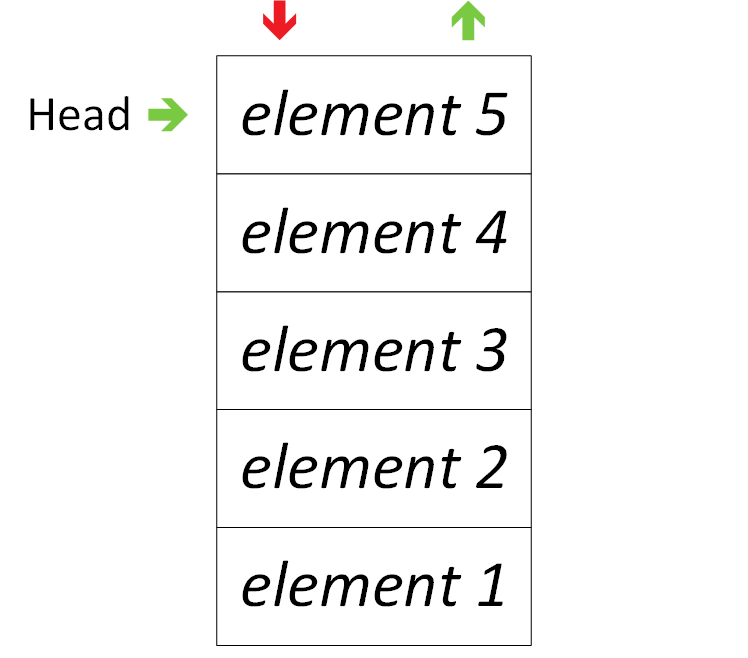
\includegraphics[scale=0.75]{Cours/Piles_1_Structure_Generale_centered.png}
\end{center}

\smallskip

Deux opérations permettent d'utiliser une pile :
\begin{itemize}
\item \TTBF{PUSH} : permettant d'\textit{empiler} une donnée supplémentaire dans la pile
\item \TTBF{POP} : permettant de \textit{dépiler} une donnée depuis la pile
\end{itemize}
On ajoute donc une donnée en l'empilant avec un \TTBF{PUSH}, et il est possible de directement y accéder, car elle est au sommet de la pile.
À l'inverse, pour accéder à une donnée tout au fond de la pile, il est nécessaire de dépiler autant d'éléments que nécessaire avec un \TTBF{POP}.\\

Voici un exemple où l'on crée une pile, puis on empile successivement $ 42 $, $ 5 $, et $ 13 $, puis, on dépile une fois (pour récupérer $ 13 $), et enfin, on empile successivement $ 37 $, $ 10 $, $ 24 $.\\

\begin{center}
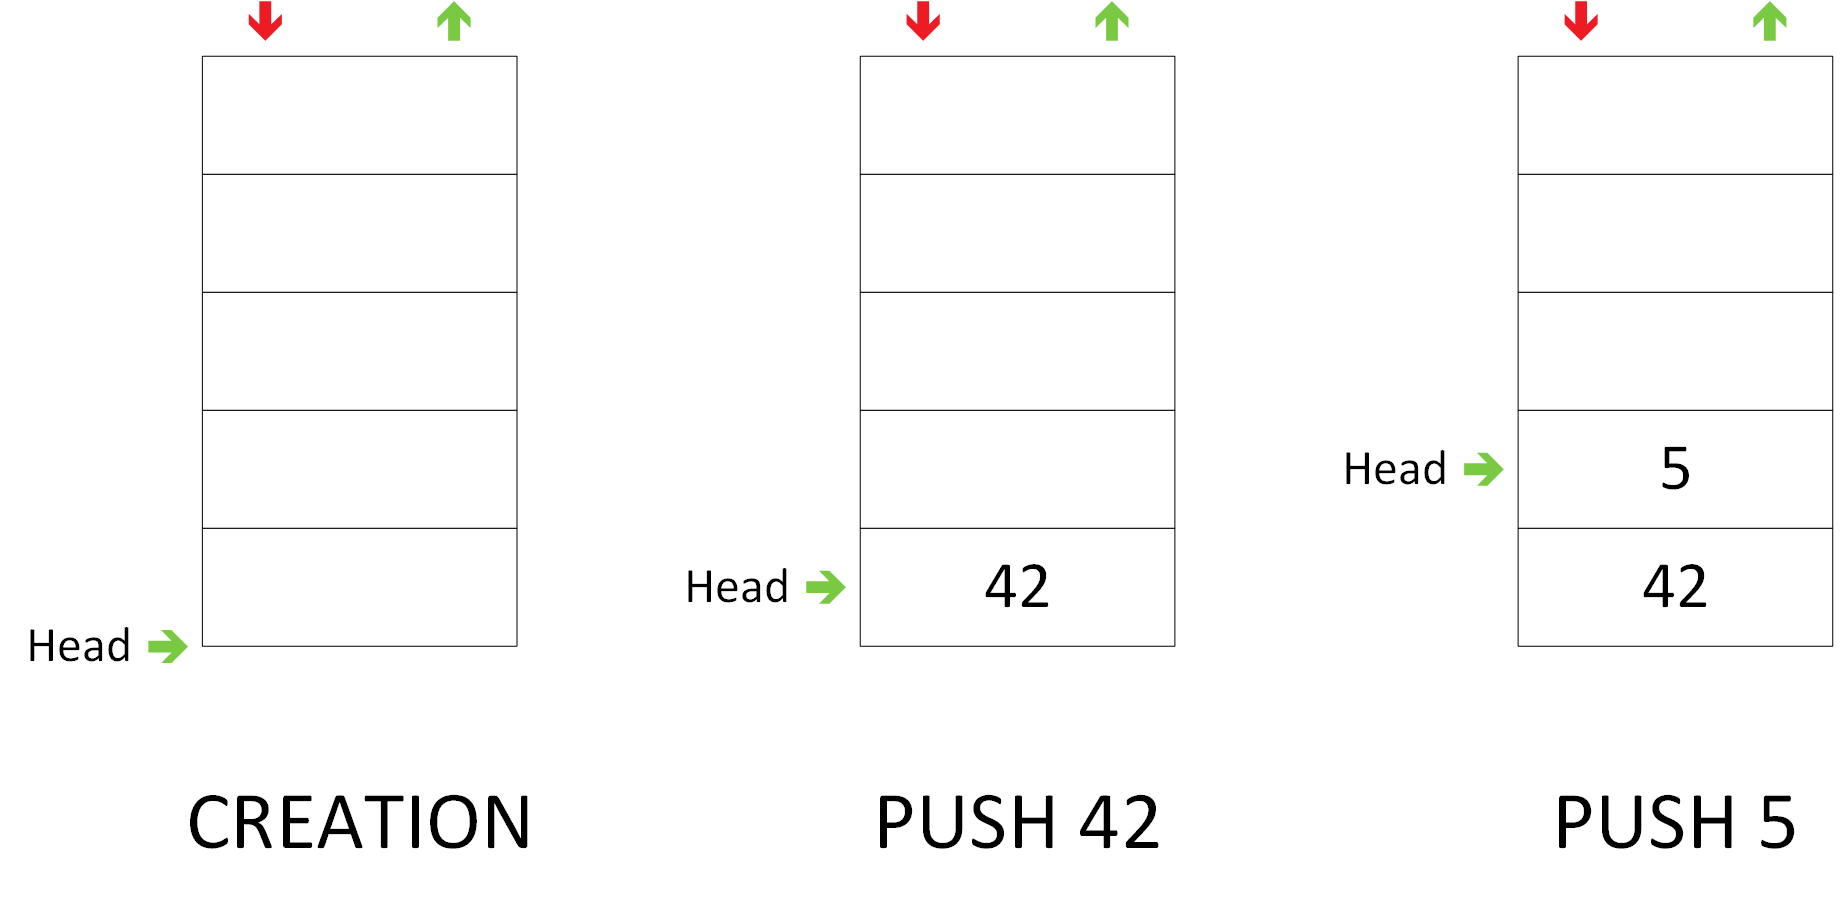
\includegraphics[scale=0.5]{Cours/Piles_2_Structure_Generale_Usage_pack_1.png}
\end{center}

\begin{center}
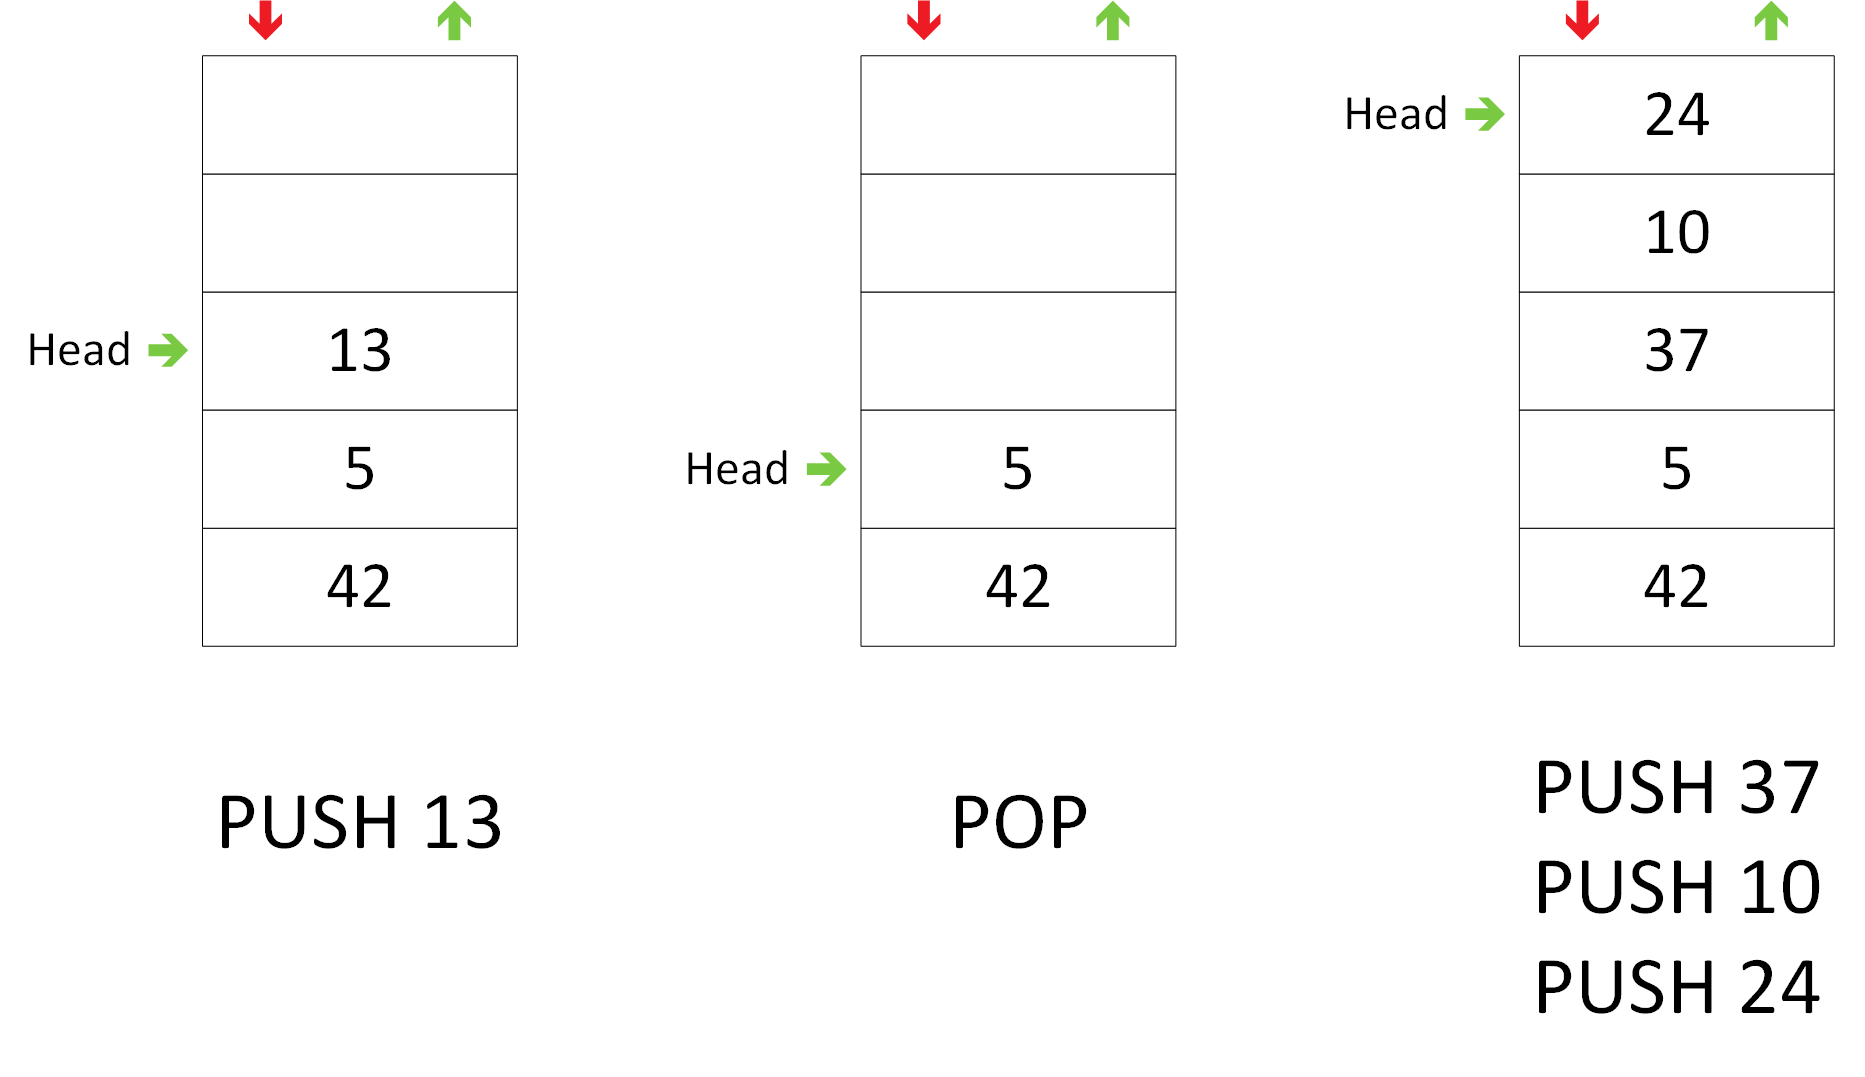
\includegraphics[scale=0.5]{Cours/Piles_2_Structure_Generale_Usage_pack_2.png}
\end{center}

\smallskip

Les piles, et surtout la contrainte d'accès aux objets, sont couramment utilisées : un camion de livraison sera d'abord rempli avec les paquets à livrer en dernier/le camion sera rempli dans l'ordre inverse de livraison (on accède d'abord aux derniers éléments chargés).

En informatique, on utilisera les piles dans certains \textit{parsers} (analyse grammaticale) pour connaître en premier l'opérateur à exécuter (opérateur binaire ? unaire ?) et dépiler par la suite le nombre exact de paramètres.
La \textit{pile d'appels} est également une convention fondamentale partagée par les processeurs et les systèmes d'exploitation permettant de passer des paramètres (et d'autres informations de contexte) aux fonctions appelées par les programmes, ou en cas d'interruption pour sauvegarder l'adresse de l'instruction qui était en cours d'exécution.\\

Afin d'implémenter une pile, il est donc nécessaire d'avoir un espace de stockage ordonné (un tableau numéroté ou une liste chaînée), et un indicateur de l'élément en haut de la pile.
Nous allons maintenant voir comment implémenter une pile avec des listes chaînées et un tableau de taille fixe.

\bigskip

%%%%%%%%%%%%%%%%%%%%%%%%%%%%%%%%%%%%%%%%%%%%%%%%%%%%%%%%%%%%
%%%%%%%%%%%%%%%%%%%%%%%%%%%%%%%%%%%%%%%%%%%%%%%%%%%%%%%%%%%%
%%%%%%%%%%%%%%%%%%%%%%%%%%%%%%%%%%%%%%%%%%%%%%%%%%%%%%%%%%%%

\subsection{Piles : implémentation avec des listes chaînées}

\bigskip

Une implémentation à l'aide d'une liste chaînée permet d'exploiter la mémoire et d'être donc beaucoup plus flexible en terme de nombre maximum d'éléments.
Le schéma suivant illustre une pile sous forme de liste chaînée en mémoire :\\

\begin{center}
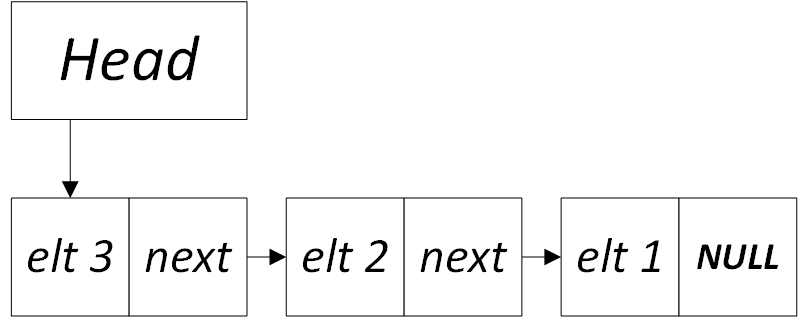
\includegraphics[scale=0.75]{Cours/Piles_3_Liste_Chainee_Structure_cas_general.png}
\end{center}

\smallskip

On y retrouve plusieurs fois la structure typique des listes chaînées (un élément et un pointeur vers l'élément suivant), ainsi qu'un pointeur indiquant le sommet de la pile (\textit{head} dans notre cas).

L'unique cas particulier concerne une pile vide : le pointeur de sommet vaut dans ce cas \TTBF{NULL}.
Il s'agit également de l'état dans lequel se trouve une pile vidée ou nouvellement créée.\\

\begin{center}
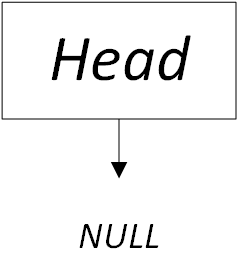
\includegraphics[scale=0.75]{Cours/Piles_3_Liste_Chainee_Structure_cas_vide.png}
\end{center}

\smallskip

L'exemple suivant montre l'évolution d'une pile au fur et à mesure des ajouts (empiler / \TTBF{PUSH}) et suppressions (dépiler / \TTBF{POP}).\\

\begin{center}
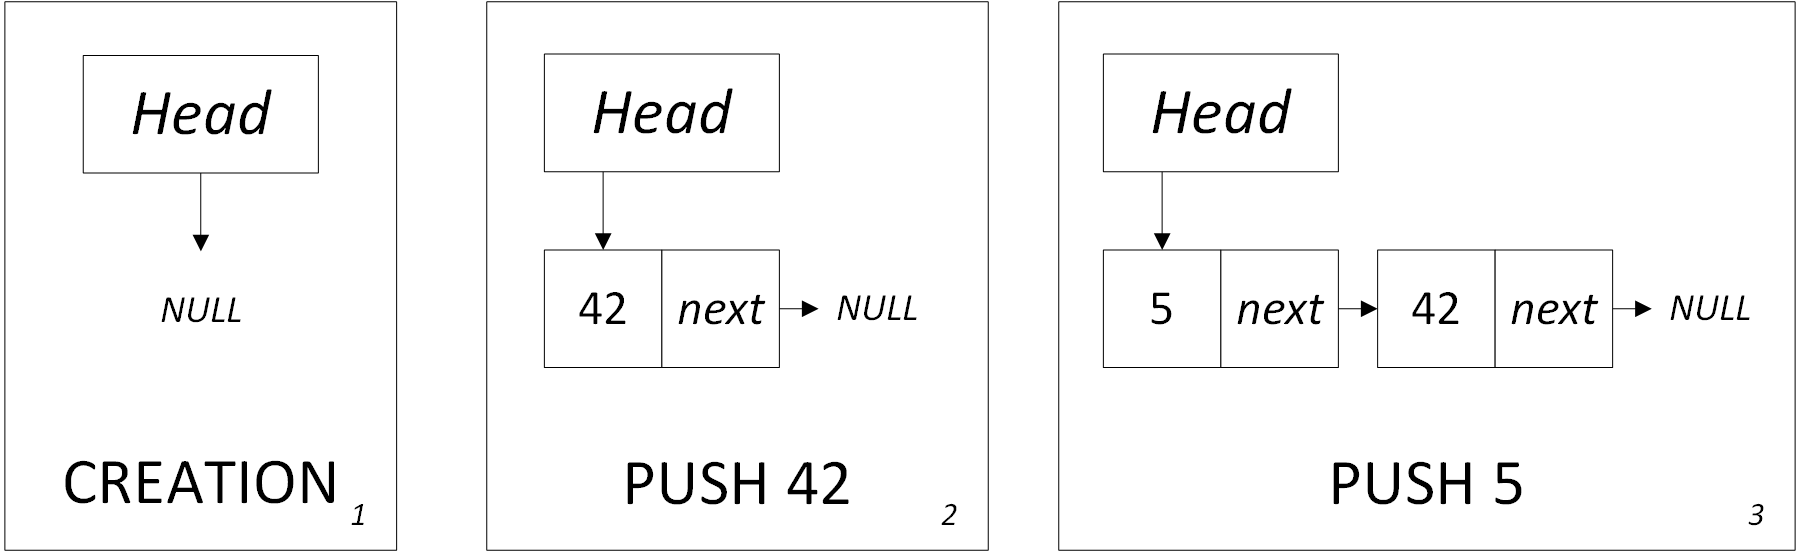
\includegraphics[scale=0.65]{Cours/Piles_4_Liste_Chainee_Usage_pack_1.png}
\end{center}

\begin{center}
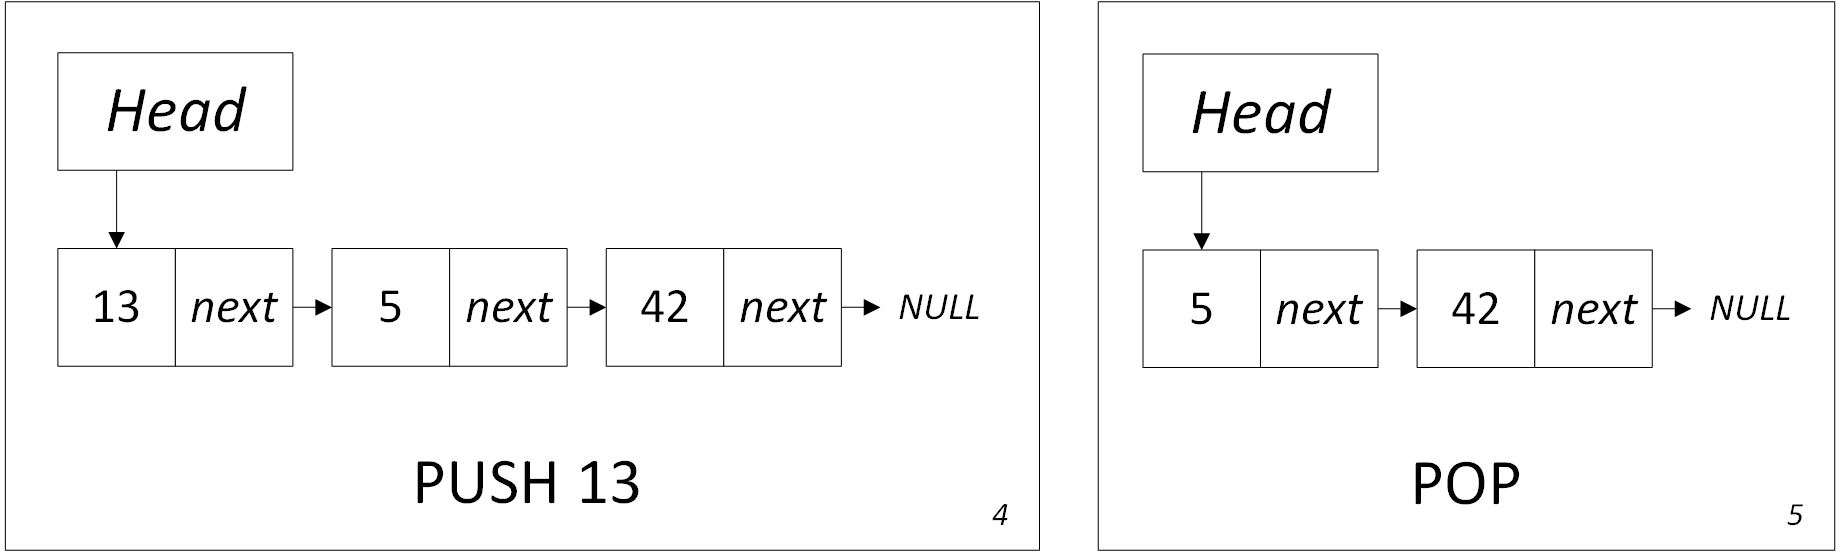
\includegraphics[scale=0.65]{Cours/Piles_4_Liste_Chainee_Usage_pack_2.png}
\end{center}

\smallskip

Les principales opérations se résument ainsi :
\begin{itemize}
\item Création : on alloue en mémoire la structure générale de la pile, et on fixe le sommet de la pile à \TTBF{NULL}.
\item Empiler : on alloue en mémoire un nouvel élément dont le pointeur \textit{next} pointe vers l'actuel élément au sommet de la pile, puis, on met à jour le pointeur de sommet de la pile vers l'adresse de ce nouvel élément.
\item Dépiler : si la pile est vide, on retourne une erreur, sinon, on récupère tout d'abord l'adresse de l'élément suivant celui au sommet, puis, on libère l'élément au sommet, puis, on met à jour le pointeur de sommet de la pile vers l'adresse de l'élément suivant.
\item Vider : on dépile successivement tous les éléments jusqu'à obtenir un sommet à \TTBF{NULL}.
\item Sommet : on renvoie le contenu de l'élément au sommet de la pile.
\end{itemize}

\bigskip

%%%%%%%%%%%%%%%%%%%%%%%%%%%%%%%%%%%%%%%%%%%%%%%%%%%%%%%%%%%%
%%%%%%%%%%%%%%%%%%%%%%%%%%%%%%%%%%%%%%%%%%%%%%%%%%%%%%%%%%%%
%%%%%%%%%%%%%%%%%%%%%%%%%%%%%%%%%%%%%%%%%%%%%%%%%%%%%%%%%%%%

\subsection{Piles : implémentation avec un tableau de taille fixe}

\bigskip

Une implémentation avec un tableau de taille fixe impose cette fois une limitation : la pile aura une taille maximale, et on peut refuser l'ajout d'un élément si la pile est déjà pleine.
La structure diffère également du fait que le tableau est alloué une seule fois lors de sa création (voire même lors de la compilation dans le cas statique).

Le schéma suivant présente la structure générale :\\

\begin{center}
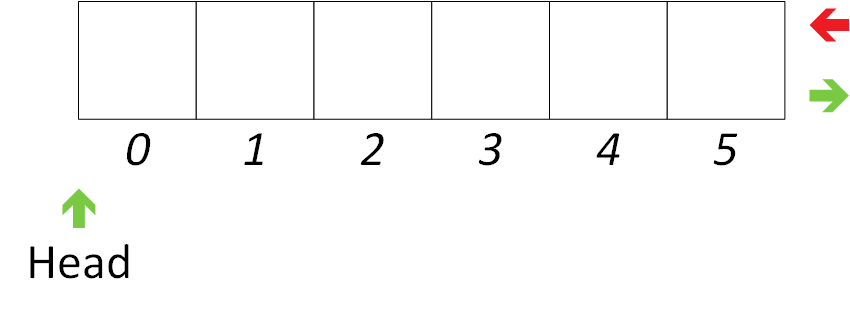
\includegraphics[scale=1]{Cours/Piles_5_Tableau_Statique_Structure.png}
\end{center}

\smallskip

On notera cette fois que plusieurs informations distinctes doivent être conservées : l'adresse du tableau, le numéro de case correspondant au sommet de la pile (\textit{head} dans notre cas), la taille du tableau (le nombre maximum d'objets pouvant être stockés), le nombre d'éléments dans le tableau.

Le schéma suivant détaille certaines informations de façon plus explicite :\\

\begin{center}
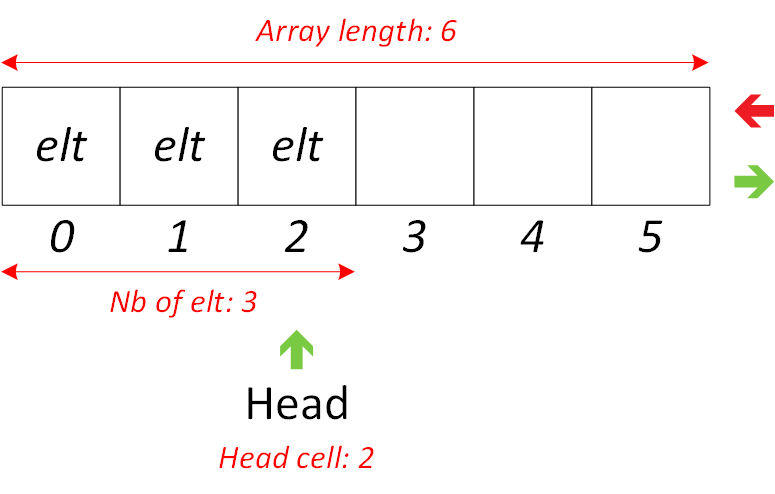
\includegraphics[scale=1]{Cours/Piles_5_Tableau_Statique_Structure_Detaillee.png}
\end{center}

\smallskip

Dans le cas d'un tableau de taille fixe, le pointeur de sommet ne peut pas utiliser la valeur \TTBF{NULL} comme indicateur de tableau vide, car cette valeur est égale à $ 0 $ (ce qui laisserait à penser que le sommet est effectivement à la case 0).
Plusieurs solutions sont possibles pour indiquer le sommet de la pile et le cas vide :

\begin{itemize}
\item On enregistre dans la structure de la pile une variable servant à compter le nombre d'éléments présents (le sommet peut donc prendre n'importe quelle valeur tant que la pile est vide).
\item On utilise un entier relatif pour indiquer le sommet, et $ -1 $ indique que la pile est vide (l'ajout d'un élément décalera le sommet à $ 0 $, c'est-à-dire la case où sera l'élément).
\item On place le sommet de la pile sur la première case non utilisée, et l'accès au premier élément se fait donc en retirant $ 1 $ au pointeur de sommet (ainsi, un sommet à la case $ 0 $ indique que la pile est vide).
Attention : dans ce cas précis, un tableau plein aura un sommet hors des cases du tableau (il ne faudra donc \textit{jamais} le déréférencer s'il atteinte une telle valeur).
\end{itemize}

\smallskip

L'exemple suivant montre l'évolution d'une pile implémentée avec un tableau fixe au fur et à mesure des ajouts (empiler / \TTBF{PUSH}) et suppressions (dépiler / \TTBF{POP}).\\

\begin{center}
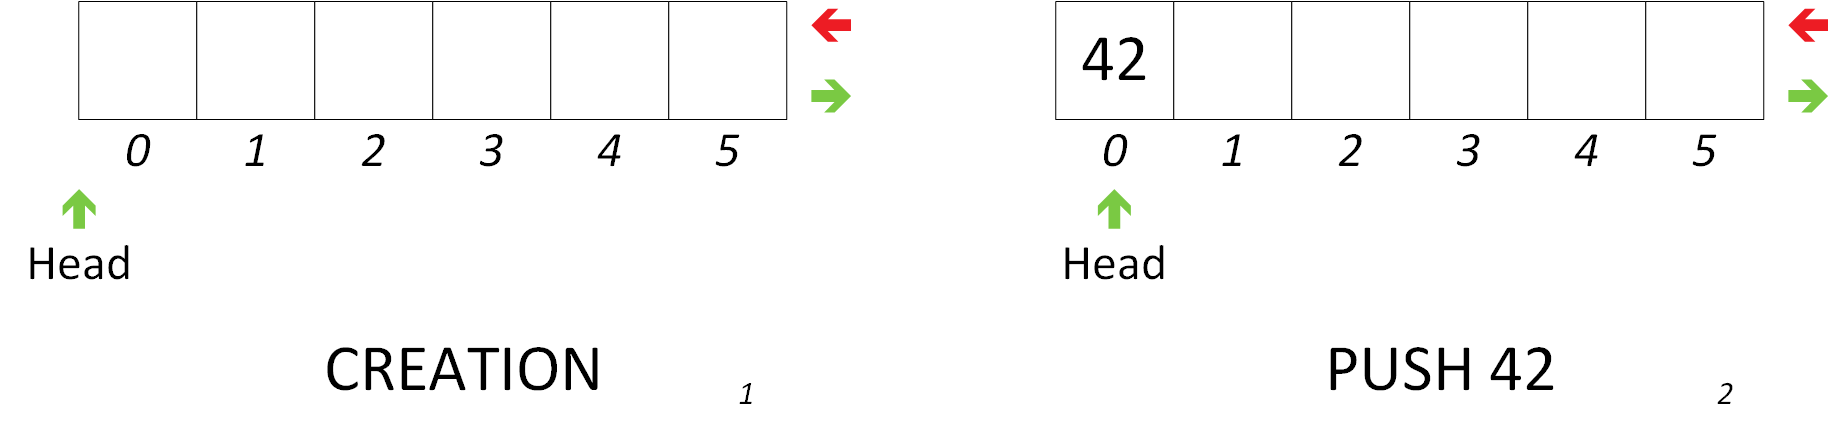
\includegraphics[scale=0.65]{Cours/Piles_6_Tableau_Statique_Usage_pack_1.png}
\end{center}

\begin{center}
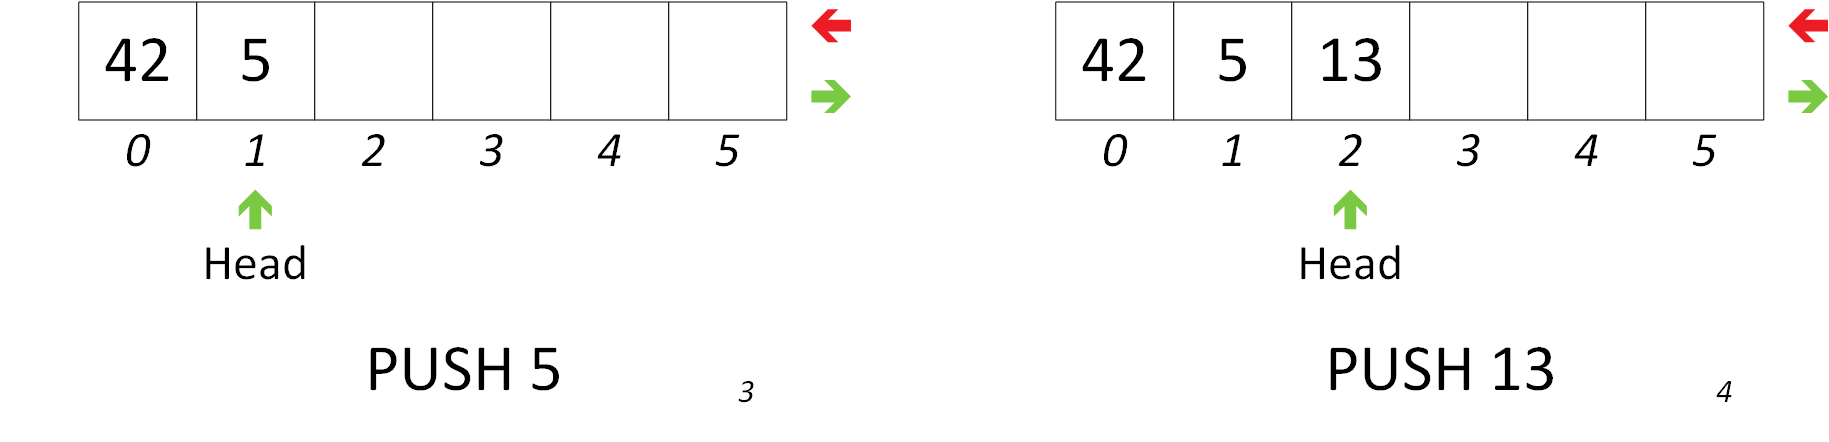
\includegraphics[scale=0.65]{Cours/Piles_6_Tableau_Statique_Usage_pack_2.png}
\end{center}

\begin{center}
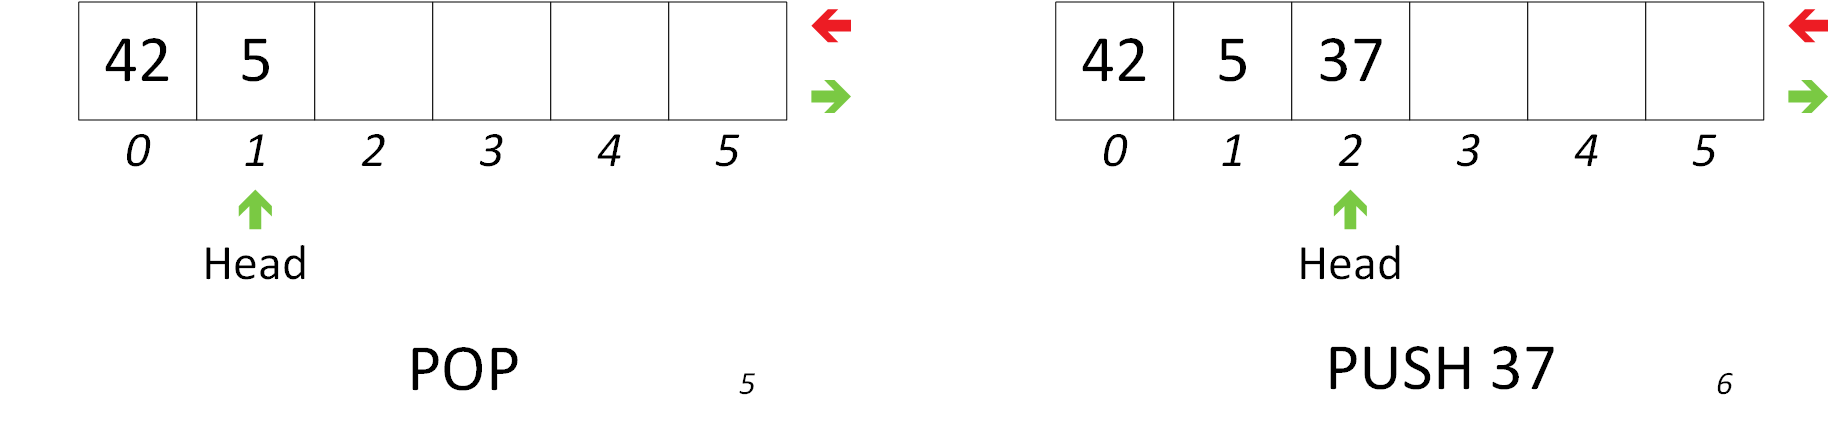
\includegraphics[scale=0.65]{Cours/Piles_6_Tableau_Statique_Usage_pack_3.png}
\end{center}

\smallskip

Les principales opérations se résument ainsi :
\begin{itemize}
\item Création : on alloue en mémoire le tableau (sauf s'il est statique), et on fixe le sommet de la pile à la valeur prévue pour démarrer ($ -1 $, $ 0 $, ou toute autre valeur choisie) [éventuellement, on met à jour le nombre d'objets dans le tableau en le fixant à $ 0 $].
\item Empiler : si le tableau est plein, on retourne une erreur, sinon, on ajoute un élément, et on décale le sommet de la pile [éventuellement, on met à jour le nombre d'objets dans le tableau].
\item Dépiler : si la pile est vide, on retourne une erreur, sinon, on réduit la valeur du sommet de la pile [éventuellement, on met à jour le nombre d'objets dans le tableau].
\item Vider : on fixe le sommet de la pile à la valeur prévue pour démarrer ($ -1 $, $ 0 $, ou toute autre valeur choisie) [éventuellement, on met à jour le nombre d'objets dans le tableau en le fixant à $ 0 $].
\item Sommet : on renvoie le dernier élément ajouté (cela dépend de comment le sommet a été implémenté !).
\end{itemize}

\setlength{\parindent}{\defaultparindent}

%
%\newpage

%%%%%%%%%%%%%%%
%% EXERCICES %%
%%%%%%%%%%%%%%%

%% Exercice 1
\section{Exercice 1 - is even}

\vspace*{0.7cm}

%% Exercice 1

%\ExoSpecs{\TTBF{CalculTVA.sh}}{\TTBF{\RenduDir/src/exo1/}}{750}{640}{\TTBF{write}}
\ExoSpecsCustom{\TTBF{exo1\_fun.php} [my\_Calculette(int, int, string)]}{\TTBF{\RenduDir/src/exo1/}}{}{}{Fonctions recommandées}{\TTBF{(Bases PHP)}, \TTBF{(Maths PHP)}, \TTBF{return}}

\vspace*{0.7cm}

\noindent \ExoObjectif{Le but de l'exercice est de créer une mini calculatrice en PHP.}

\bigskip

\noindent Vous devez écrire une fonction nommée \TTBF{my\_Calculette} qui prendra trois paramètres (deux nombres, puis l'opérateur), et renverra le résultat de l'opération désignée ou un message d'erreur.

\noindent Vous devez implémenter les 5 opérations suivantes : l'addition (symbole \TTBF{+}), la soustraction (symbole \TTBF{-}), la multiplication (lettre \TTBF{*}), la division (symbole \TTBF{/}), et le reste de la division euclidienne (symbole  \TTBF{\%}).

\noindent \`A la fin du calcul, votre fonction doit renvoyer le résultat.

\bigskip

\lstset{language=php}
\begin{lstlisting}[frame=single,title={Cas général PHP}]
<textarea cols="80" rows="25" readonly="readonly">
<?php
  require_once("exo1_fun.php");
  $my_text = my_Calculette(42, 38, "+");
  echo($my_text);
?>
</textarea>
\end{lstlisting}

\lstset{language=php}
\begin{lstlisting}[frame=single,title={Cas général PHP exécuté}]
<textarea cols="80" rows="25" readonly="readonly">
80</textarea>
\end{lstlisting}

\bigskip

\noindent Les deux premiers paramètres doivent être des entiers, et le troisième doit être une chaîne de caractères. Si ça n'est pas le cas, vous devez renvoyer le texte suivant.

\bigskip

\noindent \TTBF{Incorrect\textvisiblespace parameters\textvisiblespace type}

\bigskip

\lstset{language=php}
\begin{lstlisting}[frame=single,title={Cas d'erreur 1 : mauvais paramètres}]
<textarea cols="80" rows="25" readonly="readonly">
<?php
  require_once("exo1_fun.php");
  $my_text = my_Calculette("+", 38, 42);
  echo($my_text);
?>
</textarea>
\end{lstlisting}

\lstset{language=php}
\begin{lstlisting}[frame=single,title={Cas d'erreur 1 exécuté}]
<textarea cols="80" rows="25" readonly="readonly">
Incorrect parameters type</textarea>
\end{lstlisting}

\bigskip

\noindent Si le troisième paramètre donné n'est ni un \TTBF{+}, ni un \TTBF{-}, ni un \TTBF{*}, ni un \TTBF{/}), ni un \TTBF{\%}, alors vous devez renvoyer le message d'erreur suivant.

\bigskip

\noindent \TTBF{Unknown\textvisiblespace operator}

\bigskip

\lstset{language=php}
\begin{lstlisting}[frame=single,title={Cas d'erreur 2 : opérateur inconnu}]
<textarea cols="80" rows="25" readonly="readonly">
<?php
  require_once("exo1_fun.php");
  $my_text = my_Calculette(42, 38, "A");
  echo($my_text);
?>
</textarea>
\end{lstlisting}

\lstset{language=php}
\begin{lstlisting}[frame=single,title={Cas d'erreur 2 exécuté}]
<textarea cols="80" rows="25" readonly="readonly">
Unknown operator</textarea>
\end{lstlisting}

\bigskip

\noindent Si le deuxième paramètre donné à la division est 0, vous devez renvoyer le message d'erreur suivant.

\bigskip

\noindent \TTBF{Division\textvisiblespace by\textvisiblespace 0\textvisiblespace is\textvisiblespace forbidden}

\bigskip

\lstset{language=php}
\begin{lstlisting}[frame=single,title={Cas d'erreur 3 : division par 0}]
<textarea cols="80" rows="25" readonly="readonly">
<?php
  require_once("exo1_fun.php");
  $my_text = my_Calculette(42, 0, "/");
  echo($my_text);
?>
</textarea>
\end{lstlisting}

\lstset{language=php}
\begin{lstlisting}[frame=single,title={Cas d'erreur 3 exécuté}]
<textarea cols="80" rows="25" readonly="readonly">
Division by 0 is forbidden</textarea>
\end{lstlisting}

\bigskip

%\noindent Si le deuxième paramètre donné au modulo est 0, vous devez renvoyer le message d'erreur suivant.
%
%\bigskip
%
%\noindent \TTBF{Modulo\textvisiblespace 0\textvisiblespace is\textvisiblespace forbidden}
%
%\bigskip
%
%\lstset{language=php}
%\begin{lstlisting}[frame=single,title={Cas d'erreur 3 : division par 0}]
%<textarea cols="80" rows="25" readonly="readonly">
%<?php
%  require_once("exo1_fun.php");
%  $my_text = my_Calculette(42, 0, "%");
%  echo($my_text);
%?>
%</textarea>
%\end{lstlisting}
%
%\lstset{language=php}
%\begin{lstlisting}[frame=single,title={Cas d'erreur 3 exécuté}]
%<textarea cols="80" rows="25" readonly="readonly">
%Modulo 0 is forbidden</textarea>
%\end{lstlisting}
%
%\bigskip

\noindent Si plusieurs des problèmes précédents sont rencontrés simultanément, vous devez les gérer dans cet ordre de priorité : le problème de type en priorité, l'opérateur inconnu en second, et la division par 0 en dernier.

%\noindent Si plusieurs des problèmes précédents sont rencontrés simultanément, vous devez les gérer dans cet ordre de priorité : le problème de type en priorité, l'opérateur inconnu en second, et enfin le modulo ou la division par 0 en dernier.

\bigskip

\lstset{language=php}
\begin{lstlisting}[frame=single,title={Cas d'erreurs}]
<textarea cols="80" rows="25" readonly="readonly">
<?php
  require_once("exo1_fun.php");
  $my_text = my_Calculette("A", 42, 0);
  echo($my_text);
?>
</textarea>
\end{lstlisting}

\lstset{language=php}
\begin{lstlisting}[frame=single,title={Cas d'erreurs exécuté}]
<textarea cols="80" rows="25" readonly="readonly">
Incorrect parameters type</textarea>
\end{lstlisting}

\lstset{language=php}
\begin{lstlisting}[frame=single,title={Cas d'erreurs}]
<textarea cols="80" rows="25" readonly="readonly">
<?php
  require_once("exo1_fun.php");
  $my_text = my_Calculette(42, 0, "A");
  echo($my_text);
?>
</textarea>
\end{lstlisting}

\lstset{language=php}
\begin{lstlisting}[frame=single,title={Cas d'erreurs exécuté}]
<textarea cols="80" rows="25" readonly="readonly">
Unknown operator</textarea>
\end{lstlisting}


\newpage

%% Exercice 2
\section{Exercice 2 - Calculatrice}

\vspace*{0.7cm}

%% Exercice 2

%\ExoSpecs{\TTBF{CalculTVA.sh}}{\TTBF{\RenduDir/src/exo1/}}{750}{640}{\TTBF{write}}
\ExoSpecsCustom{\TTBF{Makefile}}{\TTBF{\RenduDir/}}{750}{640}{Outils recommandés}{\TTBF{gcc(1)}, \TTBF{ar(1)}}

\vspace*{0.7cm}

\noindent \ExoObjectif{Le but de l'exercice est de faire fonctionner l'ensemble de votre projet avec un makefile simple, et de produire une bibliothèque statique ainsi qu'une dynamique.}

\bigskip

\noindent Une bibliothèque est un ensemble de fonctions et procédures prêtes à être utilisées (ayant éventuellement des variables statiques, ou encore faisant appel à \texttt{malloc(3)}) par un utilisateur ne connaissant pas leur implémentation.
L'utilisateur développe et écrit son propre programme (utilisant un \texttt{main} pour s'exécuter) et il peut éventuellement s'appuyer sur des bibliothèques (n'ayant pas de \texttt{main}) pour réutiliser des implémentations existantes.

\bigskip

\noindent Les exercices suivants vont vous conduire à produire des fonctions manipulant des structures, afin d'offrir un service à des utilisateurs : des arbres binaires et leur interface pour les exploiter (une \texttt{API}).
Vous devez donc écrire le (ou les) \textit{makefile(s)} de votre projet et un fichier \texttt{configure} (éventuellement vide) afin de produire une bibliothèque statique nommée \TTBF{libmybintree.a} et une bibliothèque dynamique nommée \TTBF{libmybintree.so}.

\bigskip

\noindent Le \textit{makefile} que vous allez écrire rendra votre projet complet et autonome.
Pour cela, vous devez faire en sorte que plusieurs \textit{cibles} soient présentent dans le makefile (celles-ci sont rappelées dans le paragraphe suivant).
%Afin de rendre le projet parfaitement complet et autonome, vous devez écrire un \textit{makefile} répondant aux cibles indiquées dans les consignes générales (celles-ci sont rappelées dans le paragraphe suivant).

\bigskip

\noindent Plusieurs stratégies existent pour compiler avec des makefiles, l'une d'entre elle consiste à placer un makefile par dossier afin que le makefile principal appelle les suivants avec la bonne règle (par exemple : le makefile principal va appeler le makefile du dossier \textit{src} pour compiler le projet, mais le makefile principal appellera celui du dossier \textit{check} lorsque l'on demandera d'exécuter la suite de tests).

\noindent Pour ce premier contact avec les makefiles, vous pouvez vous contenter d'un seul makefile à la racine exécutant des lignes de compilation toutes prêtes sans aucune réécriture ou extension.

\bigskip

\noindent Afin de générer des bibliothèques statiques et dynamiques, vous devez compiler vos fichiers pour produire des fichiers \textit{objets} (des fichiers \TTBF{.o}), mais vous ne devez pas laisser l'étape d'\textit{édition de liens} classique se faire.
À la place, la cible \textit{static} de votre makefile devra produire une bibliothèque statique nommée \TTBF{libmybintree.a}, et la cible \textit{shared} devra produire une bibliothèque dynamique nommée \TTBF{libmybintree.so}.

\bigskip

\noindent Pour générer une bibliothèque statique (\textit{static library} en anglais), on utilise la commande \TTBF{ar} qui créée des \textit{archives}.
Pour produire la bibliothèque statique \textit{libtest.a} à partir des fichiers \textit{test1.c} et \textit{file.c}, on utilisera ces commandes :\\

\begin{tabular}{l}
\TTBF{cc -c test1.c file.c}\\
\TTBF{ar cr libtest.a test1.o file.o}\\
\end{tabular}

\bigskip

\noindent Pour générer une bibliothèque dynamique (\textit{shared library} en anglais), on utilise l'option \TTBF{-shared} du compilateur.
Pour produire la bibliothèque dynamique \textit{libtest.so} à partir des fichiers \textit{test1.c} et \textit{file.c}, on utilisera ces commandes :\\

\begin{tabular}{l}
\TTBF{cc -c test1.c file.c} \\
\TTBF{cc test1.o file.o -shared -o libtest.so} \\
\end{tabular}

\bigskip

\noindent La première commande génère des fichiers objets, et la deuxième les réunit dans un seul fichier.
Il arrivera sur certains systèmes qu'il soit nécessaire d'ajouter l'option \TTBF{-fpic} ou \TTBF{-fPIC} (\textit{Position Independent Code}) pour générer des bibliothèques dynamiques.
Gardez en tête que \textit{toutes} les bibliothèques \textbf{doivent} être préfixées par un \textit{\texttt{lib}} dans le nom des fichiers \TTBF{.a} et \TTBF{.so} générés.
Mais, lorsque l'on utiliser une bibliothèque dans un projet, on doit ignorer ce préfixe lors de la compilation et l'édition de liens.

\bigskip

\noindent Pour utiliser une bibliothèque dynamique sur votre système, plusieurs méthodes existent selon le système où vous vous trouvez.\\

\begin{itemize}
\item L'une d'entre elle consiste à ajouter le dossier contenant la bibliothèque à la variable d'environnement \TTBF{LD\_LIBRARY\_PATH} (comme pour la variable \TTBF{PATH}).
Selon votre système, il peut s'agir de la variable d'environnement \TTBF{DYLD\_LIBRARY\_PATH}, \TTBF{LIBPATH}, ou encore \TTBF{SHLIB\_PATH}.
Pour ajouter le dossier courant comme dossier contenant des bibliothèques dynamiques en plus d'autres dossiers, vous pouvez taper :\\
\TTBF{export LD\_LIBRARY\_PATH=.:/usr/lib:/usr/local/lib}
\\

\item Une autre méthode consiste à modifier le fichier \TTBF{/etc/ls.so.conf} et/ou ajouter un fichier contenant le chemin vers votre bibliothèque dans \TTBF{/etc/ld.so.conf.d/} puis à exécuter \TTBF{/sbin/ldconfig} pour recharger les dossiers à utiliser.\\

\item Enfin, vous pouvez demander les droits administrateur et installer votre bibliothèque dans \TTBF{/usr/lib} ou \TTBF{/usr/local/lib}.\\
\end{itemize}

\bigskip

\noindent \'Evidemment, à long terme, l'objectif est d'avoir une bibliothèque installée dans le répertoire \TTBF{/usr/lib}.
Mais, lors du développement, il est préférable d'utiliser la variable \TTBF{LD\_LIBRARY\_PATH}.
Pour vous assurer du fonctionnement de votre exécutable, vous pouvez utiliser \TTBF{ldd(1)} avec le chemin complet vers un exécutable.
\TTBF{ldd} vous indiquera quelles bibliothèques sont requises, et où celui-ci les trouve.
Si l'une d'entre elle n'est pas trouvée, \TTBF{ldd} vous en informera :\\

\TTBF{ldd /usr/bin/ls}

\TTBF{ldd my\_main}


\bigskip

\noindent Pour rappel voici les cibles demandées pour le \TTBF{Makefile} principal à la racine de votre projet :

\bigskip

\begin{table}
%\centering
\begin{tabular}{l p{12cm}}
\texttt{all} & \textit{[Première règle]} lance la règle \texttt{libmybintree}.\\
\texttt{clean} & supprime tous les fichiers temporaires et ceux créés par le compilateur.\\
\texttt{dist} & crée une archive propre, valide, et répondant aux exigences de rendu.\\
\texttt{distclean} & lance la règle \texttt{clean}, puis supprime les binaires et bibliothèques.\\
\texttt{check} & lance le(s) script(s) de test.\\
\texttt{libmybintree} & lance les règles \texttt{shared} et \texttt{static} \\
\texttt{shared} & compile l'ensemble du projet avec les options de compilations exigées et génère une bibliothèque dynamique.\\
\texttt{static} & compile l'ensemble du projet avec les options de compilations exigées et génère une bibliothèque statique.\\
\end{tabular}
\end{table}

\phantom{42}

\vfillFirst

\vfillLast


\newpage

%% Exercice 3
\section{Exercice 3 - Transposition de matrice}

\vspace*{0.7cm}

%% Exercice 3

%\ExoSpecs{\TTBF{CalculTVA.sh}}{\TTBF{\RenduDir/src/exo1/}}{750}{640}{\TTBF{write}}
\ExoSpecsCustom{\TTBF{exo3\_fun.php} [my\_Reduction(array, int)]}{\TTBF{\RenduDir/src/exo3/}}{}{}{Fonctions recommandées}{\TTBF{(Bases PHP)}, \TTBF{date\_format}, \TTBF{(int)}}

\vspace*{0.7cm}

\noindent \ExoObjectif{Le but de l'exercice est de calculer des réductions sur des listes de factures.}

\bigskip

\noindent A partir d'un fichier de factures émises stockées dans des tableaux, vous allez afficher ces factures en ajoutant 3 colonnes supplémentaires (le montant avec réduction appliquée, le taux de réduction, et le montant de la réduction).
Tous les montants sont stockés sous forme de centimes (300 signifie 300 centimes, soit 3 euros).

\bigskip

\noindent Pour rappel, voici comment se calculent les réductions :\\

\begin{tabular}{l c l}
Prix final après réduction : & $ Prix Final = $ & $ Prix Initial - Reduction $ \\
Réduction (20\%) depuis un prix : & $ Reduction = $ & $ Prix Initial \times 20 \div 100 $ \\
 & & \\
Prix initial si réduction (20\%) : & $ Prix Initial = $ & $ Prix Final \div 0,80 (Coef) $ \\
Coefficient de réduction de 20\% : & $ Coefficient (0,80) = $ & $ 1 - (20 \div 100) $ \\
\end{tabular}

\bigskip

\bigskip

\noindent Le tableau en entrée est de cette forme : \\

%\hspace*{-\parindent} %% BIDOUILLE
%\begin{minipage}{17cm} %% BIDOUILLE
\lstset{language=sh}
%\begin{lstlisting}[frame=single,caption={Useless code},label=useless]  % "useless" used to references
\begin{lstlisting}[frame=single,title={Tableau en entrée}]
[[ID_client (int), Date (DateTime), ID_Facture (int), Montant (int)] , [ID_client (int), Date (DateTime), ID_Facture (int), Montant (int)] , ...]
\end{lstlisting}
%\end{minipage} %% FIN BIDOUILLE

%
%% OR
%% \lstinputlisting[language=[ANSI]C]{source.c}
%% \lstinputlisting[language=Python]{source_filename.py}
%% \lstinputlisting[language=Python, firstline=37, lastline=45]{source_filename.py}
%

\bigskip

\noindent Le fichier de sortie sera de cette forme : \\

%\hspace*{-\parindent} %% BIDOUILLE
%\begin{minipage}{17cm} %% BIDOUILLE
\lstset{language=sh,basicstyle=\ttfamily \footnotesize}
\begin{lstlisting}[frame=single,title={Sortie attendue}]
ID client ; Date ; Num Facture ; Montant Final ; Montant Initial ; Taux Reduction ; Reduction
\end{lstlisting}
%\end{minipage} %% FIN BIDOUILLE

\bigskip

\noindent Exemple de structure d'entrée :

\lstset{language=sh}
\begin{lstlisting}[frame=single,title={Exemple de données en entrée}]
42421337;2006/06/06;456789;200
36153615;2018/05/30;123456;123
\end{lstlisting}

\bigskip
%\newpage

\noindent Sortie attendue pour cette entrée si on effectue une réduction de 33\% :

\lstset{language=sh}
\begin{lstlisting}[frame=single,title={Sortie attendue pour l'entrée précédente avec 33\% de réduction}]
42421337;06/06/06;456789;134;200;33;66
36153615;18/05/30;123456;83;123;33;40
\end{lstlisting}

\bigskip

\noindent (Les fichiers que nous testerons ne seront pas de mauvaise qualité : les données seront toujours correctement formatées)

\bigskip

\begin{YellowBox}
\textbf{Attention :} Certains nombres risquent de subir des virgules.
Pour éviter cela, utilisez \TTBF{((int) (x / y))} pour ne conserver que la partie entière (\texttt{123} en valeur initiale donnera donc par division \texttt{40} en réduction et \texttt{83} en valeur finale).
Attention, cette fonction tronque selon la virgule : si vous tronquez avant ou après certaines opérations, les résultats ne seront pas les mêmes !
Lors du calcul des valeurs, choisissez avec attention la ligne exacte où vous tronquerez les nombres, afin de ne pas ajouter ou retirer 1 centime.
\end{YellowBox}

\bigskip

\noindent Vous devez rendre un fichier nommé \TTBF{exo3\_fun.php} qui contiendra au moins la fonction \TTBF{my\_Reduction} qui effectuera le calcul et renverra une chaîne contenant le résultat.

\noindent La fonction prendra en paramètre un tableau qui contient lui-même des tableaux associatifs (chaque case du tableau général correspond à une facture).

\bigskip

\lstset{language=php}
\begin{lstlisting}[frame=single,title={Tableau en entrée (exo3\_data.php)}]
$tab1["ID_Client"] = 42421337;
$tab1["Date"] = new DateTime('2006-06-06');
$tab1["ID_Facture"] = 456789;
$tab1["Montant"] = 200;
$data[] = $tab1;

$tab1["ID_Client"] = 36153615;
$tab1["Date"] = new DateTime('2018-05-30');
$tab1["ID_Facture"] = 123456;
$tab1["Montant"] = 123;
$data[] = $tab1;
\end{lstlisting}

\bigskip

\lstset{language=html}
\begin{lstlisting}[frame=single,title={Appel de la fonction}]
<textarea cols="80" rows="25" readonly="readonly">
<?php
  require_once("exo3_data.php");
  require_once("exo3_fun.php");
  $my_text = my_Reduction($data, 33);
  echo($my_text);
?>
</textarea>
\end{lstlisting}

\lstset{language=html}
\begin{lstlisting}[frame=single,title={Sortie HTML attendue}]
<textarea cols="80" rows="25" readonly="readonly">
42421337;06/06/06;456789;134;200;33;66
36153615;18/05/30;123456;83;123;33;40
</textarea>
\end{lstlisting}

\bigskip

\begin{RedBoxTitle}{ATTENTION}
    Les retours à la ligne ne doivent pas être faits avec la balise \TTBF{"<br />"}, mais avec \TTBF{"\textbackslash n"}.
    (se référer à la section \hyperref[sec:AideMemoire]{Aide Mémoire})
\end{RedBoxTitle}

\newpage

%% Exercice 4
\section{Exercice 4 - Sapin}

\vspace*{0.7cm}

%% Exercice 3

%\ExoSpecs{\TTBF{CalculTVA.sh}}{\TTBF{\RenduDir/src/exo3/}}{750}{640}{\TTBF{write}}
\ExoSpecsSimple{\TTBF{my\_pintree.c}}{\TTBF{\RenduDir/src/my\_pintree.c}}{750}{640}

\vspace*{0.7cm}

\noindent \ExoObjectif{Le but de l'exercice est d'afficher un sapin en ASCII art, dont la taille varie selon le paramètre donné.}

\bigskip

\noindent Vous devez écrire un programme qui prendra un paramètre, et affichera selon ce paramètre un sapin.
\noindent Dans le cas général, affichez le sapin, et renvoyez 0.

\bigskip

\lstset{language=sh}
\begin{lstlisting}[frame=single,title={Cas général}]
$ ./my_pintree 1
 /\
/  \
____
 ||
$ echo $?
0
$ ./my_pintree 4
    /\
   /  \
  /    \
 /      \
/        \
__________
    ||
$ echo $?
0
$ ./my_pintree 5
     /\
    /  \
   /    \
  /      \
 /        \
/          \
____________
     ||
$ echo $?
0
\end{lstlisting}

\newpage

\noindent De façon précise, voici les spécifications pour les cas 1, 4, et 5 :

\bigskip

\hspace*{-\parindent} %% BIDOUILLE
\begin{minipage}{15.85cm} %% BIDOUILLE
\lstset{language=sh}
\begin{lstlisting}[frame=single,title={Cas général 1}]
 /\     1 espace / 0 espace  \
/  \    0 espace / 2 espaces \
____    4 _
 ||     1 espace 2 |
\end{lstlisting}
\end{minipage} %% FIN BIDOUILLE

\hspace*{-\parindent} %% BIDOUILLE
\begin{minipage}{15.85cm} %% BIDOUILLE
\lstset{language=sh}
\begin{lstlisting}[frame=single,title={Cas général 4}]
    /\          4 espaces / 0 espace  \
   /  \         3 espaces / 2 espaces \
  /    \        2 espaces / 4 espaces \
 /      \       1 espace  / 6 espaces \
/        \      0 espace  / 8 espaces \
__________      10 _
    ||          4 espaces 2 |
\end{lstlisting}
\end{minipage} %% FIN BIDOUILLE

\hspace*{-\parindent} %% BIDOUILLE
\begin{minipage}{15.85cm} %% BIDOUILLE
\lstset{language=sh}
\begin{lstlisting}[frame=single,title={Cas général 5}]
     /\         5 espaces / 0 espace   \
    /  \        4 espaces / 2 espaces  \
   /    \       3 espaces / 4 espaces  \
  /      \      2 espaces / 6 espaces  \
 /        \     1 espace  / 8 espaces  \
/          \    0 espace  / 10 espaces \
____________    12 _
     ||         5 espaces 2 |
\end{lstlisting}
\end{minipage} %% FIN BIDOUILLE

\bigskip

\noindent Plusieurs cas spéciaux sont à prendre en compte.\\

\noindent Tout d'abord, dans le cas où le paramètre 0 est donné, vous retournerez 0 et afficherez :

\bigskip

\lstset{language=sh}
\begin{lstlisting}[frame=single,title={Cas 0}]
$ ./my_pintree 0
/\
||
$ echo $?
0
\end{lstlisting}

\bigskip

\noindent Si aucun ou plus de 1 paramètre est donné, vous devrez afficher le message d'erreur suivant, et retourner 1 : \\

\bigskip

\noindent \TTBF{Usage:\textvisiblespace ./my\_pintree\textvisiblespace number}

\bigskip

\lstset{language=sh}
\begin{lstlisting}[frame=single,title={Cas d'erreur}]
$ ./my_pintree
Usage: ./my_pintree number
$ echo $?
1
$ ./my_pintree 0 4
Usage: ./my_pintree number
$ echo $?
1
\end{lstlisting}


%%%%%

\noindent Si un paramètre texte est donné, il sera interprété comme 0 :

\bigskip

\lstset{language=sh}
\begin{lstlisting}[frame=single,title={Cas texte}]
$ ./my_pintree blob
/\
||
$ echo $?
0
\end{lstlisting}

\bigskip

\noindent Si plusieurs paramètres sont donnés, qu'ils soient texte ou nombre, vous devez afficher le message d'erreur suivant et retourner 1.

\bigskip

\lstset{language=sh}
\begin{lstlisting}[frame=single,title={Cas texte d'erreur}]
$ ./my_pintree plop plop
Usage: ./my_pintree number
$ echo $?
1
$ ./my_pintree 3 plop
Usage: ./my_pintree number
$ echo $?
1
\end{lstlisting}


\end{document}
